\documentclass[11pt,a4paper]{article}
			\usepackage[french]{babel}
					
				\usepackage{pifont}  
				\usepackage[utf8x]{inputenc}
				\usepackage[T1]{fontenc} 
				\usepackage{lmodern}			
				\usepackage{fancyhdr}
				\usepackage{textcomp}
				\usepackage{makeidx}
				\usepackage{tabularx}
				\usepackage{multicol}
				\usepackage{multirow}
				\usepackage{longtable}
				\usepackage{color}
				\usepackage{soul}
				\usepackage{boxedminipage}
				\usepackage{shadow}
				\usepackage{framed}			
				\usepackage{array}
				\usepackage{url}
				\usepackage{ragged2e}
				\usepackage{fancybox}
				\newcommand{\cadretitre}[2]{
				  \vspace*{0.8\baselineskip}
				  \begin{center}%
				  \boxput*(0,1){%
					%\colorbox{white}{\Large\textbf{\ #1\ }}%
				  }%
				  {%
					\setlength{\fboxsep}{10pt}%
				    \Ovalbox{\begin{minipage}{.8\linewidth}\begin{center}\Large\sffamily{#2}\end{center}\end{minipage}}}%
				  \end{center}
				  \vspace*{2\baselineskip}
				  }
			
			\makeatletter
			\def\@seccntformat#1{\protect\makebox[0pt][r]{\csname the#1\endcsname\quad}}
			\makeatother

				% Permet d'afficher qqchose à une positin absolue
				\usepackage[absolute]{textpos}
				\setlength{\TPHorizModule}{1cm}
				\setlength{\TPVertModule}{\TPHorizModule}
	
				\usepackage[titles]{tocloft}
				\setlength{\cftbeforesecskip}{0.5ex}
				\setlength{\cftbeforesubsecskip}{0.2ex}
				\addto\captionsfrench{\renewcommand\contentsname{}}
				
				\usepackage[font=scriptsize]{caption}
				
				\usepackage{listings}
\lstdefinestyle{lstverb}
  {
    basicstyle=\footnotesize,
    frameround=tttt, frame=trbl, framerule=0pt, rulecolor=\color{gray},
    lineskip=-1pt,   % pour rapprocher les lignes
    flexiblecolumns, escapechar=\\,
    tabsize=4, extendedchars=true
  }
\lstnewenvironment{Java}[1][]{\lstset{style=lstverb,language=java,#1}}{}
				\ifx\pdfoutput\undefined
					\usepackage{graphicx}
				\else
					\usepackage[pdftex]{graphicx}
				\fi
				\usepackage[a4paper, hyperfigures=true, colorlinks, linkcolor=black, citecolor=blue,urlcolor=blue, pagebackref=true, bookmarks=true, bookmarksopen=true,bookmarksnumbered=true,
                pdfauthor={}, pdftitle={InitLinux - Que devez-vous revoir ?}, pdfkeywords={InitLinux - Que devez-vous revoir ?, },pdfpagemode=UseOutlines,pdfpagetransition=Dissolve,nesting=true,
				backref, pdffitwindow=true, bookmarksnumbered=true]{hyperref}
				\usepackage{supertabular}
				\usepackage[table]{xcolor}
				\usepackage{url}
				\usepackage{caption} 
				\setlength{\parskip}{1.3ex plus 0.2ex minus 0.2ex}
				\setlength{\parindent}{0pt}
				
				\makeatletter
				\def\url@leostyle{ \@ifundefined{selectfont}{\def\UrlFont{\sf}}{\def\UrlFont{\footnotesize\ttfamily}}}
				\makeatother
				\urlstyle{leo}
				
				\definecolor{examplecolor}{rgb}{0.156,0.333,0.443}
				\definecolor{definitioncolor}{rgb}{0.709,0.784,0.454}
				\definecolor{exercisecolor}{rgb}{0.49,0.639,0}
				\definecolor{hintcolor}{rgb}{0.941,0.674,0.196}
				\definecolor{tableHeadercolor}{rgb}{0.709,0.784,0.454}
				\definecolor{tablerowAltcolor}{rgb}{.866,.905,.737}
				\definecolor{tablerowAlt2color}{rgb}{.968,.976,.933}
				\definecolor{verylightgray}{rgb}{0.98,0.98,0.98}
				
				\newenvironment{fshaded}{
				\def\FrameCommand{\fcolorbox{framecolor}{shadecolor}}
				\MakeFramed {\FrameRestore}}
				{\endMakeFramed}
				
				\newenvironment{fexample}[1][]{\definecolor{shadecolor}{rgb}{.913,.913,.913}
				\definecolor{framecolor}{rgb}{.156,.333,.443}
				\begin{fshaded}}{\end{fshaded}} 
				
				\newenvironment{fdefinition}{\definecolor{shadecolor}{rgb}{.913,.913,.913}
				\definecolor{framecolor}{rgb}{.709,.784,.454}
				\begin{fshaded}}{\end{fshaded}}
				
				\newenvironment{fexercise}{\definecolor{shadecolor}{rgb}{.913,.913,.913}
				\definecolor{framecolor}{rgb}{.49,.639,0}
				\begin{fshaded}}{\end{fshaded}}
				
				\newenvironment{fhint}{\definecolor{shadecolor}{rgb}{.913,.913,.913}
				\definecolor{framecolor}{rgb}{.941,.674,.196}
				\begin{fshaded}}{\end{fshaded}}	
				
				\newcommand{\PreserveBackslash}[1]{
				\let\temp=\\#1\let\\=\temp
				}
				\let\PBS=\PreserveBackslash
				\newcolumntype{A}{>{\PBS\raggedright\small\hspace{0pt}}X}
				\newcolumntype{L}[1]{>{\PBS\raggedright\small\hspace{0pt}}p{#1}}
				\newcolumntype{R}[1]{>{\PBS\raggedleft\small\hspace{0pt}}p{#1}}
				\newcolumntype{C}[1]{>{\PBS\centering\small\hspace{0pt}}p{#1}}
				
				\makeindex
				
				\title{InitLinux - Que devez-vous revoir ?}	
			\date{}
			\author{\scriptsize{}}
			\definecolor{light-gray}{gray}{0.8}
			\renewcommand{\headrulewidth}{0pt}
			\fancyhead[L]{
				\footnotesize\textsc{Haute \'Ecole de Bruxelles}\\
	    			\footnotesize\textsc{\'Ecole Sup\'erieure d'Informatique}
			}
			\fancyhead[R]{
				\footnotesize{Bachelor en Informatique}\\
				\footnotesize{Laboratoires Java} - 
			\footnotesize{1\`ere ann\'ee}}
				\fancyfoot[L]{ }
				\fancyfoot[C]{}
				\fancyfoot[R]{\scriptsize{\textcolor{gray}{version 2014-2015 (\today)}}}
				\pagestyle{plain}
				\reversemarginpar
				\usepackage{rotating}						
				\begin{document}
					\begin{textblock}{9}(2,3.2)
						
\includegraphics[width=2cm]{../../../_templates/java/icons/logo-esi}
					\end{textblock}
				
				
				
				
				%\maketitle
				\cadretitre{TD1}{InitLinux - Que devez-vous revoir ?}
				\thispagestyle{fancy}
        \marginpar{\begin{sideways}
            \begin{minipage}[t]{1cm}
            \begin{tiny}
            
\includegraphics[width=1\linewidth,height=1\textheight,keepaspectratio=true]{../../../_templates/java/icons/cc-gris.jpg}
			\end{tiny}
			\end{minipage}
            \begin{minipage}[b]{19cm}
            \begin{tiny}
            \textcolor{gray}{Distribué sous licence Creative Commons Paternité - Partage à l'Identique 2.0 Belgique 
            (\texttt{http://creativecommons.org/licenses/by-sa/2.0/be/})
			\vspace{-1em}
			\\Les autorisations au-delà du champ de cette licence peuvent être obtenues à 
			\texttt{http://www.heb.be/esi}
			- \texttt{mcodutti@heb.be}
			}\end{tiny}
			\end{minipage}
        \end{sideways}}
            \begin{abstract}
			Cet exercice a pour but de vous situer par rapport \`a vos connaissances 
			\verb@Linux@.
		
            \par
        \end{abstract}
				\vspace{-2em}\tableofcontents
				\pagestyle{plain}
            \clearpage
            \fancyhead[L,C,R]{}
            \fancyfoot[L,C]{}
            \fancyfoot[R]{ \scriptsize{\textcolor{gray}{
				InitLinux - page \thepage}}}
				\thispagestyle{fancy}
				\pagestyle{fancy}
	   
            \section{Les commandes de base de Linux}\subsection{Quelques commandes courantes}
			
		\subparagraph{Les commandes de base} 
		
                \textcolor{white}{.} \par
             
								La commande pour :  
							
					\begin{itemize}
				
			\item voir le contenu d'un dossier (la liste de ce qu'il contient) est  \textcolor{gray}{\underline{\hspace*{2em}}} 
			\item voir le contenu d'un dossier (la liste de ce qu'il contient) au format long est  \textcolor{gray}{\underline{\hspace*{3em}}} 
			\item voir le contenu d'un dossier (la liste de ce qu'il contient), y compris les fichiers cach\'es est  \textcolor{gray}{\underline{\hspace*{3em}}} 
			\item \'editer le contenu d'un fichier est  \textcolor{gray}{\underline{\hspace*{3em}}} 
			\item changer son mot de passe est  \textcolor{gray}{\underline{\hspace*{5em}}} 
			\item se d\'econnecter de linux1 est  \textcolor{gray}{\underline{\hspace*{3em}}} 
			\item copier un fichier est  \textcolor{gray}{\underline{\hspace*{2em}}} 
			\item renommer un fichier est  \textcolor{gray}{\underline{\hspace*{2em}}} 
			\item d\'eplacer un fichier est  \textcolor{gray}{\underline{\hspace*{2em}}} 
			\item changer de dossier courant est  \textcolor{gray}{\underline{\hspace*{2em}}} 
			\item cr\'eer un r\'epertoire est  \textcolor{gray}{\underline{\hspace*{3em}}} 
			\item visualiser le contenu d'un fichier sans l'\'editer est  \textcolor{gray}{\underline{\hspace*{2em}}} 
			\item voir quel est le dossier courant (son chemin) est  \textcolor{gray}{\underline{\hspace*{2em}}} 
			\item d\'etruire un fichier est  \textcolor{gray}{\underline{\hspace*{2em}}} 
			\item d\'etruire un dossier vide est  \textcolor{gray}{\underline{\hspace*{3em}}} 
			\item d\'etruire un dossier pas forc\'ement vide est  \textcolor{gray}{\underline{\hspace*{3em}}} 
			\item d'obtenir la liste des options de la commande rm est  \textcolor{gray}{\underline{\hspace*{5em}}} 
					\end{itemize}
				
			
		\subparagraph{La ligne de commande} 
		
                \textcolor{white}{.} \par
            
					\begin{itemize}
				
			\item 
										Qu'est-ce qui permet de distinguer / s\'eparer les diff\'erentes parties d'une commande ? 
										 \textcolor{gray}{\underline{\hspace*{10em}}} 
			\item 
										Dans la commande \,\verb|rmdir|\,, combien y a-t-il de parties ?  
										 \textcolor{gray}{\underline{\hspace*{1em}}} 
			\item 
										Dans la commande \,\verb|rm dir|\,, combien y a-t-il de parties ?  
										 \textcolor{gray}{\underline{\hspace*{1em}}} 
					\end{itemize}
				Si vous avez r\'epondu correctement \`a moins de 17 questions, r\'evisez ici (\url{www.heb.be/esi/InitLinux/fr/../../TDLinux/fr/html/unit\_Bases.html})
            \par
        \section{Syst\`eme de fichiers, chemin absolu et relatif}\subsection{Exercices}
			
		\subparagraph{} 
		
                \textcolor{white}{.} \par
            La racine du syst\`eme de fichier sous Linux est
						
            \begin{itemize} 
        
            \item[ \ding{"6D} ] .
        
            \item[ \ding{"6D} ] ..
        
            \item[ \ding{"6D} ] \char`\~
        
            \item[ \ding{"6D} ] \char`\~g12345
        
            \item[ \ding{"6D} ] /
        
            \item[ \ding{"6D} ] /home
        
            \end{itemize} 
        
			
		\subparagraph{} 
		
                \textcolor{white}{.} \par
            Le(s)quel(s) de ces chemins est/sont un chemin absolu ?
						
            \begin{itemize} 
        
            \item[ \ding{"6F} ] /home/g54321/tdLinux
        
            \item[ \ding{"6F} ] \char`\~g54321/tdLinux
        
            \item[ \ding{"6F} ] g54321/tdLinux
        
            \item[ \ding{"6F} ] tdLinux
        
            \end{itemize} 
        
			
		\subparagraph{} 
		
                \textcolor{white}{.} \par
            Le(s)quel(s) de ces chemins est/sont un chemin relatif ?
						
            \begin{itemize} 
        
            \item[ \ding{"6F} ] tdLinux
        
            \item[ \ding{"6F} ] ../tdLinux
        
            \item[ \ding{"6F} ] ./.././eCours/tdLinux
        
            \item[ \ding{"6F} ] /eCours/java/tds/tdLinux
        
            \end{itemize} 
        Si vous n'avez r\'epondu correctement \`a ces 3 questions, r\'evisez ici (\url{www.heb.be/esi/InitLinux/fr/../../TDLinux/fr/html/unit\_Syst\`emeDeFichiers.html})
            \par
        \begin{figure}[hbt]
				    \begin{center}
					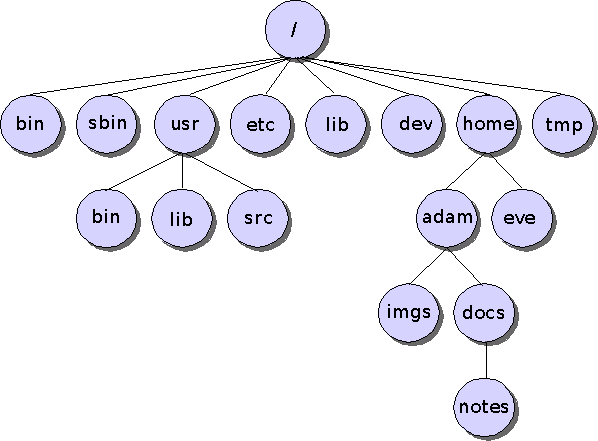
\includegraphics[width=0.8\linewidth,height=0.8\textheight,keepaspectratio=true]{/home/clr/Documents/Cours/DEV1Q2/InitLinux/fr/image/arborescenceUnix.png}
						\end{center}
                
                    \caption[arborescenceUnix.png]{arborescenceUnix.png}
                \end{figure}
                    
			    
			    [source : franceftars.us.62-152-34-99.ppa.listkom.ru]
        
            \par
        
			
		\subparagraph{La ligne de commande} 
		
                \textcolor{white}{.} \par
            
							Supposons que le r\'epertoire courant est le dossier personnel \,\verb|/home/adam|\,
					\begin{itemize}
				
			\item 
										Quelle commande permet de supprimer le r\'epertoire \,\verb|imgs|\, et son contenu en utilisant un chemin absolu ?
										 \textcolor{gray}{\underline{\hspace*{16em}}} 
			\item 
										Quelle commande permet de supprimer le r\'epertoire \,\verb|imgs|\, et son contenu en utilisant un chemin relatif ?
										 \textcolor{gray}{\underline{\hspace*{10em}}} 
			\item 
										Quelle commande permet de cr\'eer un r\'epertoire \,\verb|imgs|\, 
										dans le r\'epertoire \,\verb|eve|\, en utilisant un chemin relatif ?
										 \textcolor{gray}{\underline{\hspace*{16em}}} 
			\item 
										Quelle commande permet de cr\'eer un fichier \,\verb|mesImages|\, 
										dans le r\'epertoire \,\verb|imgs|\, du r\'epertoire \,\verb|eve|\, en utilisant un chemin absolu ?
										 \textcolor{gray}{\underline{\hspace*{16em}}} 
			\item 
										Quelle commande permet de copier ce fichier \,\verb|mesImages|\, 
										que vous venez de cr\'eer dans le r\'epertoire courant en utilisant que des chemins relatifs ?
										 \textcolor{gray}{\underline{\hspace*{16em}}} 
					\end{itemize}
				\begin{figure}[hbt]
				    \begin{center}
					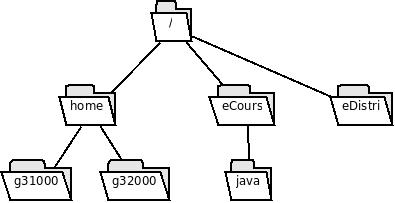
\includegraphics[width=0.8\linewidth,height=0.8\textheight,keepaspectratio=true]{/home/clr/Documents/Cours/DEV1Q2/InitLinux/fr/image/fs.jpeg}
						\end{center}
                
                    \caption[fs.jpeg]{fs.jpeg}
                \end{figure}
                    
            \par
        
			
		\subparagraph{La ligne de commande} 
		
                \textcolor{white}{.} \par
            
							Supposons que le r\'epertoire courant est le dossier personnel \verb@/home/g31000@
					\begin{itemize}
				
			\item 
										Quelle commande permet de supprimer le r\'epertoire \verb@java@ et son contenu en utilisant un chemin absolu ?
										 \textcolor{gray}{\underline{\hspace*{16em}}} 
			\item 
										Quelle commande permet de supprimer le r\'epertoire \verb@java@ et son contenu en utilisant un chemin relatif ?
										 \textcolor{gray}{\underline{\hspace*{16em}}} 
			\item 
										Quelle commande permet de cr\'eer un r\'epertoire \verb@tds@ 
										dans le r\'epertoire \verb@g32000@ en utilisant un chemin relatif ?
										 \textcolor{gray}{\underline{\hspace*{16em}}} 
			\item 
										Quelle commande permet de cr\'eer un fichier \verb@Ex.java@ 
										dans le r\'epertoire \verb@tds@ 
										du r\'epertoire \verb@g32000@ en utilisant un chemin relatif ?
										 \textcolor{gray}{\underline{\hspace*{16em}}} 
			\item 
										Quelle commande permet de copier ce fichier \verb@Ex.java@ 
										que vous venez de cr\'eer dans le r\'epertoire courant en utilisant que des chemins relatifs ?
										 \textcolor{gray}{\underline{\hspace*{16em}}} 
			\item 
										Quelle commande permet de lister au format long le dossier personnel en utilisant un chemin absolu ?
										 \textcolor{gray}{\underline{\hspace*{5em}}} 
					\end{itemize}
				Si vous avez fait plus de 2 erreurs, r\'evisez ici (\url{www.heb.be/esi/InitLinux/fr/../../TDLinux/fr/html/unit\_Syst\`emeDeFichiers.html})
            \par
        \section{La ligne de commande}\subsection{La ligne de commande}
			
		\subparagraph{Exercice} 
		
					\textcolor{white}{.} \par
				
            \par
        
					\begin{enumerate}
				
			\item 
            Dans votre dossier td3, copiez le fichier \par
				\verb@monfichieraunomtellementlongquilmeparaitpeuprobabledeletaper2xsanserreur@
            qui se trouve dans le dossier \verb@/eCours/java/td/td3@.
          
			\item Affichez le contenu de ce fichier en \'evitant de retaper son nom.
					\end{enumerate}
				
			
		\subparagraph{Exercices} 
		
					\textcolor{white}{.} \par
				
            \par
        
					\begin{enumerate}
				
			\item 
            Copiez dans votre r\'epertoire td3 tous les fichiers du r\'epertoire 
            \verb@/eCours/java/td/td3@ dont la deuxi\`eme lettre est un '\verb@x@'.
          
			\item 
            Copiez dans votre r\'epertoire tdLinux tous les fichiers du r\'epertoire
            \verb@/eCours/java/td/td3@ dont l'extension est \verb@.java@ 
            (c'est possible sans passer par un \,\verb|cd /eCours/java/td/td3|\,)
          
			\item 
            Listez le contenu des r\'epertoires des \'etudiants (pour rappel, les r\'epertoires des \'etudiants sont ceux 
            qui se trouvent dans \verb@/home@ et qui commencent par un '\verb@g@').
          
			\item 
            Listez le contenu des r\'epertoires des professeurs (pour rappel, les  
            r\'epertoires des professeurs sont ceux qui se trouvent dans \verb@/home@ et qui sont compos\'es de 3 lettres).
          
					\end{enumerate}
				
			
		\subparagraph{S\'election multiple} 
		
                \textcolor{white}{.} \par
            La commande \verb@rm td*.java@ supprime le(s) fichier(s) :
						
            \begin{itemize} 
        
            \item[ \ding{"6F} ]  
							td.java
						
        
            \item[ \ding{"6F} ]  
							td2
						
        
            \item[ \ding{"6F} ]  
							td2.java
						
        
            \item[ \ding{"6F} ]  
							td3Prepa.java
						
        
            \item[ \ding{"6F} ]  
							td3.java
						
        
            \item[ \ding{"6F} ]  
							td10.java
						
        
            \end{itemize} 
        
			
		\subparagraph{} 
		
                \textcolor{white}{.} \par
            La commande \verb@rm td?.java@ supprime le(s) fichier(s) :
						
            \begin{itemize} 
        
            \item[ \ding{"6F} ]  
              td.java
						
        
            \item[ \ding{"6F} ]  
							td2
						
        
            \item[ \ding{"6F} ]  
							td2.java
						
        
            \item[ \ding{"6F} ]  
							td3Prepa.java
						
        
            \item[ \ding{"6F} ]  
							td3.java
						
        
            \item[ \ding{"6F} ]  
							td10.java
						
        
            \end{itemize} 
        Si vous vous \^etes tromp\'e dans un de ces exercices, r\'evisez ici (\url{www.heb.be/esi/InitLinux/fr/../../TDLinux/fr/html/LigneDeCommande\_learningObject1.html})
            \par
        \section{Les permissions}\subsection{Les permissions}
			
		\subparagraph{Exercices} 
		
					\textcolor{white}{.} \par
				
            \par
        
					\begin{enumerate}
				
			\item Visualisez le propri\'etaire des fichiers de votre dossier personnel.
			\item Cr\'eez un r\'epertoire \verb@tdLinux@ dans votre dossier personnel ;
			\item Visualisez le propri\'etaire des fichiers de votre dossier \verb@tdLinux@.
					
					\end{enumerate}
				
			
		\subparagraph{Exercices} 
		
					\textcolor{white}{.} \par
				
            \par
        
					\begin{enumerate}
				
			\item Visualiser les groupes auxquels vous appartenez.
			\item Visualiser le groupe auquel appartient votre dossier \verb@tdLinux@.
			\item Quel est votre groupe principal ? 
			\item Quels sont les groupes auxquels appartient votre professeur ?
			\item Avez-vous un groupe en commun avec lui ?
			\item Quel(s) groupe(s) Linux avez-vous en commun avec les autres \'etudiants de votre groupe ESI ?
			\item Changez le groupe de  votre dossier \verb@tdLinux@ 
					pour que les enseignants puissent avoir des permissions diff\'erentes de celles des \'etudiants .
					\end{enumerate}
				
			
		\subparagraph{Exercices} 
		
					\textcolor{white}{.} \par
				
            \par
        
					\begin{enumerate}
				
			\item Visualisez vos fichiers et d\'eterminez \`a quel groupe ils appartiennent.
			\item Cr\'eez un fichier de test et modifiez le groupe auquel il appartient.
					\end{enumerate}
				Si vous avez fait plus de 2 erreurs, r\'evisez ici (\url{www.heb.be/esi/InitLinux/fr/../../TDLinux/fr/html/unit\_Permissions.html})
            \par
        
			
		\subparagraph{D\'eterminez les bonnes permissions} 
		
                \textcolor{white}{.} \par
              
							Remplissez les blancs avec la permission correcte (r, w, x ou -). 
							Il s'agit de trouver la permission minimale \`a mettre pour r\'epondre \`a la demande.   
						
					\begin{itemize}
				
			\item 
									Pour un fichier Java, la permission la plus ad\'equate est
									 \textcolor{gray}{\underline{\hspace*{1em}}}  \textcolor{gray}{\underline{\hspace*{1em}}}  \textcolor{gray}{\underline{\hspace*{1em}}} 
			\item 
									Pour la version compil\'ee (le bytecode), la permission la plus ad\'equate est
									 \textcolor{gray}{\underline{\hspace*{1em}}}  \textcolor{gray}{\underline{\hspace*{1em}}}  \textcolor{gray}{\underline{\hspace*{1em}}} 
			\item 
									Le fichier qui contient (l'ex\'ecutable de) la machine virtuelle a probablement comme permisson
									 \textcolor{gray}{\underline{\hspace*{1em}}}  \textcolor{gray}{\underline{\hspace*{1em}}}  \textcolor{gray}{\underline{\hspace*{1em}}} 
					\end{itemize}
				
			
		\subparagraph{Exercice } 
		
					\textcolor{white}{.} \par
				
            \par
          
					Soit le fichier \verb@Max.java@ de la capture d'\'ecran ci-dessous.  
				
            \par
        \begin{figure}[hbt]
				    \begin{center}
					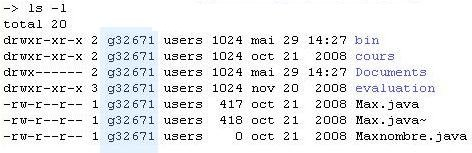
\includegraphics[width=0.8\linewidth,height=0.8\textheight,keepaspectratio=true]{/home/clr/Documents/Cours/DEV1Q2/InitLinux/fr/image/ls-l.jpg}
						\end{center}
                
                    \caption[Contenu d\'etaill\'e d'un dossier]{Contenu d\'etaill\'e d'un dossier}
                \end{figure}
                    
					Est-ce qu'un professeur peut l'\'editer ? 
				
            \par
        \fcolorbox{gray}{verylightgray}{\parbox{\textwidth}{\textcolor{verylightgray}{\LARGE  Non ! Le droit d'écriture n'est accordé qu'au propriétaire.  }}} {\footnotesize\emph{(la r\'eponse est disponible dans la version en ligne)}\par} 
			
		\subparagraph{D\'eterminez les bonnes permissions} 
		
                \textcolor{white}{.} \par
            
							Soit le fichier "Max.java" de la capture d'\'ecran ci-dessus.
							
							On voudrait que l'\'etudiant \verb@g32671@ puisse travailler  
							normalement, que les autres \'etudiants ne puissent pas tricher sur  
							lui mais que les professeurs puissent lire son travail.   
						
					\begin{itemize}
				
			\item 
									Quel groupe faut-il donner au fichier ?
									\par
				 \textcolor{gray}{\underline{\hspace*{10em}}} 
			\item 
									Quelle commande permet de donner ce groupe au fichier ?
									\par
				 \textcolor{gray}{\underline{\hspace*{3em}}}  \textcolor{gray}{\underline{\hspace*{10em}}}  \textcolor{gray}{\underline{\hspace*{10em}}} 
			\item 
									Quelles permissions minimales donner au fichier ?                
									\par
				 \textcolor{gray}{\underline{\hspace*{1em}}}  \textcolor{gray}{\underline{\hspace*{1em}}}  \textcolor{gray}{\underline{\hspace*{1em}}}  \textcolor{gray}{\underline{\hspace*{1em}}}  \textcolor{gray}{\underline{\hspace*{1em}}}  \textcolor{gray}{\underline{\hspace*{1em}}}  \textcolor{gray}{\underline{\hspace*{1em}}}  \textcolor{gray}{\underline{\hspace*{1em}}}  \textcolor{gray}{\underline{\hspace*{1em}}} 
			\item 
									Quelle commande permet de donner ces permissions au fichier ?
									\par
				 \textcolor{gray}{\underline{\hspace*{3em}}}  \textcolor{gray}{\underline{\hspace*{2em}}}  \textcolor{gray}{\underline{\hspace*{10em}}} 
					\end{itemize}
				
			
		\subparagraph{Exercice} 
		
					\textcolor{white}{.} \par
				
            \par
          
					Reprenez les permissions affich\'ees dans la capture d'\'ecran ci-dessous 
					et exprimez-les avec un nombre de 3 chiffres.  
				
            \par
        \begin{figure}[hbt]
				    \begin{center}
					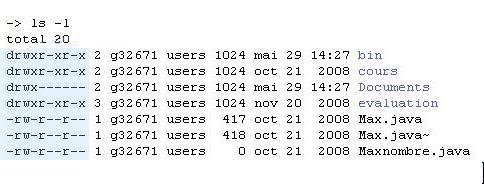
\includegraphics[width=0.8\linewidth,height=0.8\textheight,keepaspectratio=true]{/home/clr/Documents/Cours/DEV1Q2/InitLinux/fr/image/ls-l-permissions.jpg}
						\end{center}
                
                    \caption[Contenu d\'etaill\'e d'un dossier]{Contenu d\'etaill\'e d'un dossier}
                \end{figure}
                    \clearpage
			
		\subparagraph{Permissions par d\'efaut} 
		
					\textcolor{white}{.} \par
				
            \par
        
					\begin{enumerate}
				
			\item Si ce n'est pas encore fait, cr\'eez un dossier "tdLinux".
			\item Cr\'eez-y un fichier vide.
			\item Demandez les d\'etails du fichier (propri\'etaire, groupe, permission)
					\end{enumerate}
				 
					On constate qu'un nouveau fichier appartient \`a celui qui l'a cr\'e\'e 
					(on s'en doute) et au groupe principal du cr\'eateur. 
					Il y a aussi des permissions par d\'efaut (plut\^ot permissives dans notre cas).  
				
            \par
        
			
		\subparagraph{Modifier les permissions} 
		
					\textcolor{white}{.} \par
				
            \par
          
					Vous savez que la commande qui permet de modifier les permissions d'un fichier est 
					\,\verb|chmod|\,.  
				
            \par
          
					Prenez le temps de \textbf{lire} 
					la page de \textbf{manuel} de cette commande.   
				
            \par
        
			
		\subparagraph{Exercices} 
		
					\textcolor{white}{.} \par
				
            \par
        
					\begin{enumerate}
				
			\item Cr\'eez un fichier \verb@brol@ dans le dossier \verb@tdLinux@ avec quelques mots.
			\item Faites en sorte que personne d'autre ne puisse en voir le contenu.
			\item Faites en sorte que tout le monde puisse voir son contenu mais pas le modifier. 
			\item 
					  Faites en sorte que les autres \'etudiants ne puissent pas voir son contenu mais les professeurs bien. 
					  Attention, pour ce faire, il faut pouvoir distinguer les \'etudiants des enseignants; et donc, distinguer les groupes.
					
					\end{enumerate}
				
			
		\subparagraph{Exercices} 
		
					\textcolor{white}{.} \par
				
            \par
          
					Modifiez les droits de votre dossier \verb@tdLinux@ et, si n\'ecessaire, 
					des fichiers qui s'y trouvent pour que tout le monde puisse  
				
            \par
        
					\begin{enumerate}
				
			\item voir quels fichiers s'y trouvent mais sans pouvoir lire le contenu de ces fichiers;
			\item modifier le contenu d'un des fichiers mais pas supprimer ce fichier;
			\item supprimer un fichier mais pas modifier son contenu.
					\end{enumerate}
				
			
		\subparagraph{Les permissions} 
		
                \textcolor{white}{.} \par
            Remplissez les blancs avec la permission minimale correcte (r, w, x ou -),
					\begin{enumerate}
				
			\item 
									pour que le r\'epertoire \verb@/home/gxxxxx/td3@ 
									permette \`a un autre \'etudiant d'y cr\'eer le fichier  
									\verb@/home/gxxxxx/td3/fichier@\par
				 \textcolor{gray}{\underline{\hspace*{1em}}}  \textcolor{gray}{\underline{\hspace*{1em}}}  \textcolor{gray}{\underline{\hspace*{1em}}}  \textcolor{gray}{\underline{\hspace*{1em}}}  \textcolor{gray}{\underline{\hspace*{1em}}}  \textcolor{gray}{\underline{\hspace*{1em}}}  \textcolor{gray}{\underline{\hspace*{1em}}}  \textcolor{gray}{\underline{\hspace*{1em}}}  \textcolor{gray}{\underline{\hspace*{1em}}} 
			\item 
									pour que le r\'epertoire \verb@/home/gxxxxx/td3@ 
									permette \`a un autre \'etudiant d'acc\'eder au fichier  
									\verb@/home/gxxxxx/td3/fichier@
									dont il connait le chemin
									\par
				 \textcolor{gray}{\underline{\hspace*{1em}}}  \textcolor{gray}{\underline{\hspace*{1em}}}  \textcolor{gray}{\underline{\hspace*{1em}}}  \textcolor{gray}{\underline{\hspace*{1em}}}  \textcolor{gray}{\underline{\hspace*{1em}}}  \textcolor{gray}{\underline{\hspace*{1em}}}  \textcolor{gray}{\underline{\hspace*{1em}}}  \textcolor{gray}{\underline{\hspace*{1em}}}  \textcolor{gray}{\underline{\hspace*{1em}}} 
					\end{enumerate}
				
			
		\subparagraph{} 
		
                \textcolor{white}{.} \par
            Modifiez les permissions 
					\begin{itemize}
				
			\item 
									pour que le fichier \verb@/home/gxxxxx/td3/fichier@ 
									puisse \^etre lu et modifi\'e par votre professeur et vous m\^eme mais seulement lu par les autres \'etudiants 
									\par
				 \textcolor{gray}{\underline{\hspace*{3em}}}  \textcolor{gray}{\underline{\hspace*{1em}}}  \textcolor{gray}{\underline{\hspace*{1em}}}  \textcolor{gray}{\underline{\hspace*{1em}}}  \textcolor{gray}{\underline{\hspace*{16em}}} 
			\item 
								  \`A quel groupe ce fichier doit-il appartenir ?
									\par
				 \textcolor{gray}{\underline{\hspace*{10em}}} 
			\item 
								  Quelle commande permet de modifier le groupe du fichier afin de l'adapter \`a ce qui est demand\'e ci-dessus ?
									\par
				 \textcolor{gray}{\underline{\hspace*{3em}}}  \textcolor{gray}{\underline{\hspace*{10em}}} 
					\end{itemize}
				
			
		\subparagraph{S\'election multiple} 
		
                \textcolor{white}{.} \par
            Parmi les propositions suivantes, lesquelles repr\'esentent des chemins absolus ?
            \begin{itemize} 
        
            \item[ \ding{"6F} ] \verb@/usr/local/java/@
        
            \item[ \ding{"6F} ] \verb@/home/g31000/td3@
        
            \item[ \ding{"6F} ] \verb@g31000/td3@
        
            \item[ \ding{"6F} ] \verb@~/td3@
        
            \item[ \ding{"6F} ] \verb@td3@
        
            \item[ \ding{"6F} ] \verb@~g31000/td3@
        
            \end{itemize} 
        Si vous avez fait plus de 2 erreurs, r\'evisez ici (\url{www.heb.be/esi/InitLinux/fr/../../TDLinux/fr/html/unit\_Permissions.html})
            \par
        \section{Commandes}\subsection{Commandes}
			
		\subparagraph{Exercices} 
		
					\textcolor{white}{.} \par
				
					\begin{enumerate}
				
			\item 
							Comment trouver les programmes Java
							du TD4
							o\`u vous avez d\'ej\`a utilis\'e un "switch" ?
						
			\item 
							Comment trouver,
							parmi \textbf{tous}
							les programmes Java
							que vous avez d\'ej\`a \'ecrits,
							ceux qui utilisent des bool\'eens ?
						
					\end{enumerate}
				
			\fcolorbox{gray}{verylightgray}{
			\begin{minipage}[c][2cm][c]{\textwidth}\textcolor{verylightgray}{X}\end{minipage}
		}\par\medskip
            \par
         Si vous vous \^etes tromp\'e, r\'evisez ici (\url{www.heb.be/esi/InitLinux/fr/../../TDLinux/fr/html/Grep\_learningObject1.html})
            \par
        
			
		\subparagraph{Exercice} 
		
					\textcolor{white}{.} \par
				
            \par
        
          Trouvez avec la commande 
          \verb@find@
          tous les fichiers Java que vous avez d\'ej\`a \'ecrits.
        
            \par
        
			\fcolorbox{gray}{verylightgray}{
			\begin{minipage}[c][1cm][c]{\textwidth}\textcolor{verylightgray}{X}\end{minipage}
		}\par\medskip
          Nous avons \'ecrit pour vous une classe
          \verb@Color@
          mais nous ne savons plus tr\`es bien
          o\`u nous l'avons stock\'ee.
          Nous nous rappelons juste l'avoir mise
          quelque part dans 
          \verb@/eCours@.
          Pouvez-vous la retrouver pour nous ?
        
            \par
        
			\fcolorbox{gray}{verylightgray}{
			\begin{minipage}[c][1cm][c]{\textwidth}\textcolor{verylightgray}{X}\end{minipage}
		}\par\medskip Si vous vous \^etes tromp\'e, r\'evisez ici (\url{www.heb.be/esi/InitLinux/fr/../../TDLinux/fr/html/Find\_learningObject1.html})
            \par
        \section{Redirections}\subsection{Entr\'ees et sorties standards}
			
		\subparagraph{Exercice} 
		
					\textcolor{white}{.} \par
				
            \par
        
					\begin{enumerate}
				
			\item 
						Reprenez votre programme qui affiche
						des suites de nombres et plus pr\'ecis\'ement
						celui qui affiche la suite appel\'ee :
						"le pas croissant".
						Ex\'ecutez-le pour
						afficher les 1000 premiers nombres de cette suite.
					
			\item 
						Sauvez le r\'esultat dans un fichier
						pour pouvoir l'examiner \`a votre aise.
						\textbf{Rappel} :
						pour examiner le contenu d'un fichier,
						inutile de passer par un \'editeur,
						la commande
						\verb@more@
						suffit.
					
			\item 
						Est-ce que le nombre 15007 en fait partie ?
						(aide : vous vous rappelez de la commande
						\verb@grep@ ?)
					
					\end{enumerate}
				Si vous vous \^etes tromp\'e, r\'evisez ici (\url{www.heb.be/esi/InitLinux/fr/../../TDLinux/fr/html/unit\_Redirections.html})
            \par
        \subsection{Rediriger l'entr\'ee}
			
		\subparagraph{Exercice} 
		
					\textcolor{white}{.} \par
				
            \par
        
					On vous demande d'afficher,
					parmi les 1000 premiers nombres 
					de la suite des pas croissants,
					tous ceux qui sont des multiples de 5.
					Combien y en a-t-il ?
				
            \par
        Si vous vous \^etes tromp\'e, r\'evisez ici (\url{www.heb.be/esi/InitLinux/fr/../../TDLinux/fr/html/unit\_Redirections.html})
            \par
        \subsection{Les tubes (pipes en anglais)}
			
		\subparagraph{Exercice} 
		
					\textcolor{white}{.} \par
				
            \par
        
					\begin{enumerate}
				
			\item 
              Utilisez un pipe pour afficher
              parmi les 1000 premiers nombres 
              de la suite des pas croissants,
              tous ceux qui sont des multiples de 5.
            
			\item 
              Supprimez du programme
              \verb@Multiples5@
              la ligne finale qui affiche 
              le nombre de multiples trouv\'es. 
            
			\item 
              Relancez votre commande de l'exercice pr\'ec\'edent.
              Vous ne voyez plus, \`a la fin,
              le nombre de multiples, ce qui est normal.
              Quelle enchainement de commandes
              permet d'afficher ce nombre
              (et uniquement ce nombre) ?
              Rappelez-vous,
              il existe une commande Linux qui "compte". 
            
			\item 
              Affichez,
              parmi les 1000 premiers nombres 
              de la suite des pas croissants,
              tous ceux qui contiennent un 0.
            
					\end{enumerate}
				 Si vous vous \^etes tromp\'e, r\'evisez ici (\url{www.heb.be/esi/InitLinux/fr/../../TDLinux/fr/html/unit\_Redirections.html})
            \par
        \subsection{Rediriger les erreurs}
			
		\subparagraph{Exercice} 
		
					\textcolor{white}{.} \par
				
            \par
        
					Les professeurs se demandent combien
					d'\'etudiants ont d\'ej\`a copi\'e chez eux
					le fichier 
					\verb@Multiple5.java@.
					Pouvez-vous indiquer la (suite de) commande(s)
					qui permet de r\'epondre \`a la question ?
				
            \par
         Si vous vous \^etes tromp\'e, r\'evisez ici (\url{www.heb.be/esi/InitLinux/fr/../../TDLinux/fr/html/unit\_Redirections.html})
            \par
        \section{Les filtres Linux}\subsection{Les filtres Linux}
			
		\subparagraph{Exercice 1 - Nombre de connexions d'un utilisateur} 
		
					\textcolor{white}{.} \par
				
            \par
        
					Trouvez un enchainement de commandes
					qui permet de donner le nombre de connexions
					d'un utilisateur donn\'e.
				
            \par
        
					Il existe de nombreuses fa\c cons de r\'esoudre
					cet exercice. 
					Celle \`a laquelle nous pensons fait intervenir :
					\verb@grep@,
					\verb@wc@,
					et \verb@who@.
				
            \par
        
			
		\subparagraph{Exercice 2 - Nombre de PC connect\'es} 
		
					\textcolor{white}{.} \par
				
            \par
        
					Trouvez un enchainement de commandes
					qui permet de donner le nombre de PC
					connect\'es \`a linux1.
					Ce n'est pas exactement le nombre d'utilisateurs
					car un utilisateur pourrait \^etre connect\'e
					sur plusieurs machines.
				
            \par
        
					\`A nouveau,
					il existe de nombreuses fa\c cons de r\'esoudre
					cet exercice. 
					Celle \`a laquelle nous pensons fait intervenir
					la commande 
					\verb@tr -s ' '@
					qui supprime plusieurs occurences
					cons\'ecutives d'un m\^eme caract\`ere
					facilitant ainsi la s\'election par colonne
					de la commande 
					\verb@cut@.
				
            \par
        
			
		\subparagraph{Exercice 3 - Droits sur les dossiers personnels} 
		
					\textcolor{white}{.} \par
				
            \par
        
					Trouvez un enchainement de commandes
					qui permet de donner 
					le nombre de professeurs
					qui ont donn\'e le droit \`a ceux qui
					ne font pas partie de leur groupe
					d'entrer dans leur dossier personnel.
				
            \par
         Si vous vous \^etes tromp\'e, r\'evisez ici (\url{www.heb.be/esi/InitLinux/fr/../../TDLinux/fr/html/Filtres\_learningObject1.html})
            \par
        \section{Gestion des processus}\subsection{Gestion des processus}
			
		\subparagraph{Exp\'erimentation - La boucle infinie} 
		
					\textcolor{white}{.} \par
				
            \par
        
					\begin{enumerate}
				
			\item 
						\'Ecrivez un programme minimal 
						contenant une boucle infinie
						\begin{Java}
	while(true){}
						\end{Java}
			\item 
						Visualisez vos processus en cours en utilisant la commande 
						\verb@ps u@.
					
			\item 
						Ouvrez une seconde fen\^etre putty, et ex\'ecutez-y 
						votre boucle infinie.
						Ex\'ecutez \`a nouveau la commande 
						\verb@ps u@
						dans la premi\`ere fen\^etre.
					
			\item 
						Retrouvez le processus correspondant au programme 
						qui cycle (son PID)
						et tuez-le en utilisant la commande kill
						avec les bons param\`etres. Quel nom a le programme \`a tuer ?
						
            \par
        
						Sur linux1,
						le syst\`eme tue les processus apr\`es un temps d\'efini
						d'utilisation du CPU (timeout). Il se pourrait donc
						qu'il s'arr\^ete avant l'effet de votre action ;
						ce n'est pas le moment de s'endormir ;-).
						
            \par
        
			\item 
						Lancez une deuxi\`eme ex\'ecution et suspendez votre programme 
						par \verb@Ctrl-z@.
						V\'erifiez l'\'etat du processus stopp\'e par la commande 
						\verb@ps@
						(\verb@man ps@ et recherchez 
						la signification du champ 
						\verb@STAT@).
					
			\item 
						Reprenez le processus interrompu en envoyant le signal 
						SIGCONT (via la commande kill) 
						et v\'erifiez son nouvel \'etat avant qu'il ne soit \'eject\'e par 
						le syst\`eme \`a cause du \guillemotleft timeout\guillemotright .
					
			\item 
						Une deuxi\`eme mani\`ere de reprendre un processus suspendu
						est de taper la commande
						\verb@fg num@ 
						(faites un \verb@man bash@),
						cela doit \^etre fait dans la console dans laquelle vous 
						avez tap\'e \verb@Ctrl-z@.
						Le num\'ero \verb@num@
						est fourni par le syst\`eme lorsque le processus 
						a \'et\'e suspendu par \verb@Ctrl-z@.
						
            \par
        
						Essayez aussi \verb@fg@ 
						pour reprendre le dernier processus suspendu.
						
            \par
        
					\end{enumerate}
				 Si vous vous \^etes tromp\'e, r\'evisez ici (\url{www.heb.be/esi/InitLinux/fr/../../TDLinux/fr/html/Processus\_learningObject1.html})
            \par
        
				\end{document}
			